\section{METHODS}

\subsection{Digital Phantom}
Based on the fiber geometries of the digital phantom 
created for the \gls*{hardi} 
reconstruction Challenge held in ISBI 2013 
(San Francisco, US), we simulated high resolution 
(0.5mm isotropic) T1 (TE/TR=10/1500ms) and T2 
(TE/TR=90/5000ms) images, as well as two \gls*{dmri}
images (1.0mm isotropic, $b$=1200, 1 B0 image) with
32 and 64 evenly-distributed directions.
Diffusion is modeled by a restricted and a hindered
compartment, similar to \cite{assaf_composite_2005}.
The phantom includes \gls*{wm} fiber bundles,
\gls*{gm} and \gls*{csf}. Physical properties
(T1/T2 times in sec) used in simulation are
($0.832\pm0.010$ / $79\times10^{-3}\pm0.6\times10^{-3}$)
for \gls*{wm},
($1.331\pm0.013$ / $110\times10^{-3}\pm2.0\times10^{-3}$) for
\gls*{gm} and ($3.5\pm0.1$ / $0.25\pm0.01$) for \gls*{csf}.

\subsection{Theory-based synthetic distortion}
\label{sec:distortion}
\Gls*{fmb} methodologies use a map
of the field in the scanner. More precisely, the
phase difference between two subsequent samplings
of the fieldmap. With that information, it is possible
to compute the theoretical displacement that each
voxel undergoes, the so-called \gls*{vsm}. The
most prominent feature of this \gls*{vsm} is that all
the shifts have the same orientation (parallel to the
phase-encoding direction of the \gls*{epi}) and their
magnitude and direction depend on the \gls*{epi} 
gradient increments (or \emph{blips}), and the actual
phase difference at the voxel.

In order to create a realistic distortion, we
generated a synthetic phase-difference map 
consistent with the phantom, using the 
tools distributed with the \emph{FSL} package 
\cite{jenkinson_fsl_2012}  and
standard parameters ($\Delta$TE=2.46~ms. for the
field mapping and \emph{effective dwell time} of 
0.77~ms. for the \gls*{epi}).
We defined two regions of smooth dephasing and 
computed the corresponding \gls*{vsm}. Amplitude
of the dephasing maps can be modulated, enabling
us to evaluate the impact of the distortion magnitude.
We generated several \glspl*{vsm} with increasing
maximum shifts, ranging 3.80-7.60~mm, covering the
typical range of distortion observed in real datasets.

From these synthetic \glspl*{vsm}, we generated
the corresponding distorted \glspl*{dwi}, in two opposed
phase-gradient encoding directions. The second simulated
``acquisition'' of the same phantom was necessary 
for evaluating \gls*{reb} methods.

In summary, we generated 
a full gold-standard containing realistic T1 and T2
at high resolution, \glspl*{dwi} acquired in two
different phase encoding directions, and a ground-truth
\gls*{dwi} data, which is not available for real datasets
(\autoref{fig:phantom}).


\begin{figure}[thpb]
   \centering
   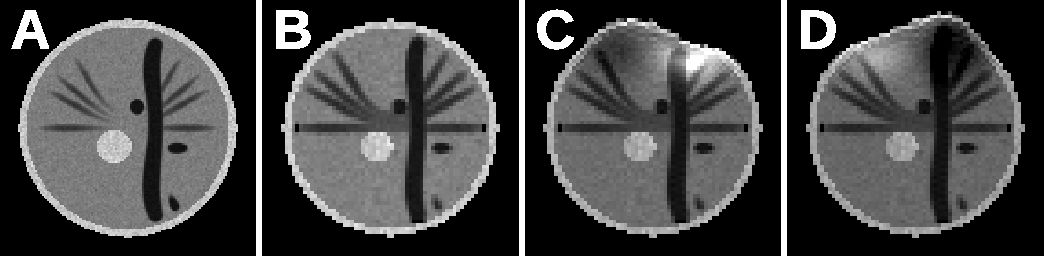
\includegraphics[width=0.95\columnwidth]{Fig01-Phantom}
   \caption{Ground-truth digital phantom.
   A) T2-weighted image; B) undistorted \textit{b0} volume;
   C, D) distorted \textit{b0} volumes with opposed phase 
   encoding directions, maximum displacement of 3.80~mm.}
   \label{fig:phantom}
\end{figure}

\subsection{Correction methods}
\label{sec:correction}
Three out of four methods presented in \autoref{sec:intro}
were tested on the evaluation framework. 

\Gls*{fmb} correction
is essentially the same as the one used for generating the 
distortion, on the inverse direction. Normally distributed 
noise was added to the fieldmap (for a signal-to-noise 
ratio of 20dB) before correction.

For \Gls*{reb} correction, we made use of the implementation found 
in \emph{FSL} (\texttt{topup})
that demands for the \textit{b0} of the reverse-encoding simulation.
In this second case, the \gls*{vsm} is inferred from the differences
between the two corresponding \textit{b0}.

Finally, for evaluating \Gls*{t2b},
we fine-tuned \emph{ANTs} \cite{avants_ants:_2013},
in order to register \textit{b0} to T2. To this end, we used a
multi-resolution scheme with 3 levels of subsampling and smoothing,
mutual information metric, and symmetric diffeomorphic transform 
(\texttt{SyN}). Several configurations of kernel widths for the 
regularization smoothers were tested, and finally selected 
0.5/1.0 voxels (gradient/deformation fields, respectively) 
for its best result. Additionally, undistorted images are 
corrected for dropout using the determinant
of the Jacobian of the deformation field.

\subsection{Evaluation}
\label{sec:evaluation}
The original phantom, one distorted version, and
the corrected instances are then connected to a
\gls*{dwi} reconstruction and tractography pipeline.
Additionally, the original tissue probability maps
are also distorted and corrected to provide tractography
with the required \gls*{wm} masks.
These maps are also used in a final assessment module.

The framework provides two different options for
\gls*{dwi} reconstruction and deterministic tractography.
Firstly, \emph{Diffusion Toolkit} \cite{wang_diffusion_2007}
for \gls*{dti}, is configured with 10 random
seeds per voxel by default. Secondly, \emph{MRTrix}
\cite{tournier_mrtrix:_2012} for \gls*{hardi}, with
default parameters set to use constrained spherical
deconvolution, maximum harmonic order of 6, and 150000
desired tracks.
For both options, the seeding regions can be set to use
either the distorted-corrected \gls*{wm} mask, or the 
regions used to generate the ground-truth. This second
seeding strategy mimics the usual procedure on real 
data, where regions are typically mapped from the
anatomically correct T1.

The evaluation framework is completed by automated 
assessment modules. We evaluated three characteristics
of the correction methods. 
Firstly, we assessed the geometrical correctness
reporting overlap indices of three tissue
probability maps (namely \gls*{csf}, \gls*{wm},
and \gls*{gm}), weighting the average by tissue
volumes.
Secondly, to evaluate the quality of the actual 
signal dropout correction, we studied the 
similarity volume by volume computing the $\ell_1$-norm
correlation index. We report this score
on the \textit{b0} and the average of the remaining \gls*{dwi}
volumes. Thirdly, we studied the impact on the
connectivity matrices reporting the number of
false positives (inexistent connections in the
gold-standard) and false negatives (or connections
lost).